\documentclass[12pt,english]{extarticle}
\usepackage{mathptmx}
\usepackage[T1]{fontenc}
%\usepackage[latin9]{inputenc}
\usepackage[letterpaper]{geometry}
\geometry{verbose,tmargin=2.0cm,bmargin=2.0cm,lmargin=2.5cm,rmargin=2.5cm,headheight=1.5cm,headsep=1.5cm,footskip=1.5cm}
\setcounter{tocdepth}{2}
\setlength{\parskip}{\smallskipamount}
\setlength{\parindent}{0pt}
\usepackage{color}
\usepackage{prettyref}
\usepackage{float}
\usepackage{amsmath}
\usepackage{graphicx}
\usepackage{subfigure}
\usepackage{amssymb}
\usepackage{fancyvrb}
\usepackage{hyperref}
\usepackage{babel}
\usepackage{makeidx}

\usepackage{listings,xcolor}
\lstset{
        language={[90]Fortran},
        extendedchars=false,          % non-English characters
        lineskip=2pt,
        backgroundcolor=\color{white},
        basicstyle=\tt\scriptsize\color{black},
        commentstyle=\tt\color{green!40!black},
        keywordstyle=\tt\color{blue},
        stringstyle=\tt\color{magenta},
        showspaces=false,             % underline spaces in the codes
        showstringspaces=false,       % underline spaces only in a string
        showtabs=false,               % underline tabs in the codes
        identifierstyle=\tt\color{red!60!black},
        numberstyle=\tiny\color{black},
        numbersep=14pt,               % how far the line-numbers are from the code
        texcl=false,                  % comments in LaTeX if true
        emph={                        % keywords to be highlighted
%               subroutine, return,
%               end
        },
        emphstyle=\sf\bfseries\color{red!50!black}\fcolorbox{orange!40!white}{.},
        numbers=left,
        rulecolor=\color{green},
        frame=single
%        tabsize=2,                    % set default tab-size to 2 spaces
%        frame=shadowbox, rulesepcolor=\color{blue}
}

\makeindex

\begin{document}

\title{User's Guide of the Program \textsc{UniMoVib} \\
\vspace{10 mm} (Ver. 1.3.0) \vspace{30 mm} \\
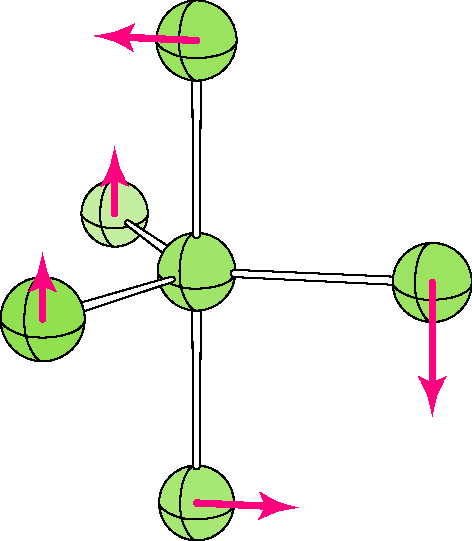
\includegraphics[width=50.0mm]{fig/logo} \vspace{30 mm} }

\date{\today}

\author{Wenli Zou \\ \vspace{5mm}
\href{mailto:qcband@gmail.com}{qcband@gmail.com} \\ \vspace{10mm}}

\maketitle
\setcounter{page}{0}
\thispagestyle{empty}

\begin{center}
\emph{Institute of Modern Physics, Northwest University, Xi'an, Shaanxi, China}
\end{center}

\pagebreak{}

\tableofcontents{}

\pagebreak{}

\section{About \textsc{UniMoVib}} \label{part:about}

\textsc{UniMoVib} is a \textsc{Uni}fied interface for \textsc{Mo}lecular \textsc{Vib}rational harmonic frequency calculations.

The \textsc{UniMoVib} program was originally written by Wenli Zou in FORTRAN 77 during 2014 and 2015 at Southern Methodist University (SMU), Dallas,
Texas, within the framework of the \textsc{LocalMode} program (now \href{https://sites.smu.edu/dedman/catco/}{\textsc{LModeA}}) of the Computational and Theoretical Chemistry Group (\href{https://sites.smu.edu/dedman/catco/}{CATCO}) of SMU. This work was
supported by the NSF grants CHE 1152357 and CHE 1464906. Guidance from the late Dr. Dieter Cremer is acknowledged. After being rewritten in Fortran 90 in the spring of 2017, \textsc{UniMoVib} has been released as a stand-alone program.

\subsection{Features} \label{sec:feature}
\index{{Features}@{Features}}

\begin{itemize}
\item Calculate harmonic vibrational frequencies and (optional) I.R. intensities from Hessian, coordinates, and other related data generated by quantum chemistry programs or by the user manually. \\
    Nearly 30 quantum chemistry programs have been supported (see Section \ref{sec:inp-contrl}), although some of them may do these calculations much better.
\index{{Quantum chemistry program}@{Quantum chemistry program}!MOPAC}
\item Analyze point group of geometry and irreducible representations (\emph{irreps.}) of normal modes in full symmetry (for \emph{irreps.}: closed-shell molecule only). \\
    Symmetry analysis is based on the symmetry subroutines from \textsc{Mopac} 7.1, which is fully in the public domain (at \href{http://openmopac.net/Downloads/Downloads.html}{openmopac.net} and \href{https://sourceforge.net/projects/mopac7/}{sourceforge.net}).
\item Thermochemistry calculation uses the point group in full symmetry, and the results are printed in Gaussian-style (for detailed explanations, see Foresman and Frisch, \emph{Exploring Chemistry With Electronic Structure Methods}, Ed.2, Gaussian Inc., Pittsburgh, PA, \textbf{1996}, p.66).
\item Generalized subsystem vibrational analysis (GSVA) to calculate intrinsic fragmental vibrations (see \textit{J. Chem. Theory Comput.} 14(5), 2558-2569, 2018).
\item Save a \textsc{Molden} file for animation of normal modes.
\item Set up isotopic masses, temperature, pressure, scale factor and/or experimental frequencies, and so on.
\item Can be used as a third party module for frequency and thermochemistry calculations in a quantum chemistry program, especially when non-Abelian group is not supported therein.
\end{itemize}

\subsection{Symmetry} \label{sec:symm}
\index{{Symmetry}@{Symmetry}}

The point group symmetries supported are listed in Table \ref{tab:symm}.

\begin{table}[H]
\caption{Available Point Groups.}\label{tab:symm}
\small\centering
\begin{tabular}{ll}
\hline\hline
$C_{n}$           & n = 1\ldots 8 \\
$C_s$, $C_{nv}$   & n = 2\ldots 8 \\
$C_i$, $C_{nh}$   & n = 2\ldots 8 \\
$D_{n}$           & n = 2\ldots 8 \\
$D_{nd}$          & n = 2\ldots 7 \\
$D_{nh}$          & n = 2\ldots 8 \\
$S_{n}$           & n = 4, 6, 8 \\
Others            & $R_3$, $T$, $T_d$, $T_h$, $O$, $O_h$, $I$, $I_h$, $C_{\infty v}$, $D_{\infty h}$ \\
\hline\hline
\end{tabular}
\end{table}

Two point groups will be printed by the program, \emph{i.e.} the molecular point group of ``\verb|Electronic| \verb|Wavefunctions|'' and the molecular point group of ``\verb|Nuclear & Total Wavefunctions|''. The former does not depend on isotopic masses whereas the latter does. The latter point group symmetry should be used to analyze vibrations and do thermochemistry calculations. However, some quantum chemistry programs use the former symmetry by mistake, and therefore the \emph{irreps.} cannot be correctly analyzed and the Gibbs free energy may be wrong. A extreme case is the fullerence $^{12}$C$_{59}{}^{13}$C, which has $I_h$ symmetry for electronic wavefunctions, but $C_1$ for nuclear wavefunctions and total wavefunctions. If $I_h$ is used in thermochemistry calculations, the error in the Gibbs free energy will be as large as 2.5 kcal/mol!

\pagebreak{}


\section{Compiling and Running} \label{part:setting}

\subsection{Compiling the program} \label{sec:install}
\index{{Installation}@{Installation}}

\verb|$ cd $UniMoVib/src| \\
\verb|$ make |

A Fortran90 compiler is required, which is defined in \verb|Makefile|.


\subsection{Running the program} \label{sec:run}
\index{{Running}@{Running}}

Double-click the binary program \verb|unimovib.exe|, and type in the name of input file (MS-Windows only), \\ \\
or \\
in the terminal, type in \\
\verb|$ ./unimovib.exe | \\
and then type in the name of input file (if no input file name provided, the default name \verb|job.inp| will be assumed), \\ \\
or \\
in the terminal, type in \\
\verb|$ ./unimovib.exe -b < input > output | \\

In the last way, one can prepare a batch script to perform a series of calculations.

\pagebreak{}


\section{Input description} \label{part:input}

The input options are grouped by namelists, which are ended by \verb|$END|.
These groups may be given in any order as desired. Before each \verb|$| symbol
there should be at least one space.

The input file is case-insensitive except the data file names specified in the \verb|$QCData|
group (section \ref{sec:inp-qcdata}).

\subsection{\texttt{\$Contrl} group} \label{sec:inp-contrl}
\index{{\texttt{\$Contrl} group}@{\texttt{\$Contrl} group}}

This group specifies the type of calculation. Keywords:

\bigskip{}\bigskip{}
\index{{\texttt{\$Contrl} group}@{\texttt{\$Contrl} group}!\texttt{QCProg}}
\index{{Quantum chemistry program}@{Quantum chemistry program}}
\verb|QCProg="XXXX"|: \verb|XXXX| is either the name of quantum chemistry program to calculate Hessian matrix and vibrational frequencies or the file format containing those data. The following programs or formats are supported:
\begin{itemize}
\index{{Quantum chemistry program}@{Quantum chemistry program}!Gaussian}
\item \verb|Gaussian| (default).
\index{{Quantum chemistry program}@{Quantum chemistry program}!GAMESS}
\item \verb|GAMESS| (\verb|GAMESS-US| and \verb|GAMESSUS| are synonyms).
\index{{Quantum chemistry program}@{Quantum chemistry program}!Firefly}
\item \verb|Firefly| (\verb|PCGamess| and \verb|PC-Gamess| are synonyms).
\index{{Quantum chemistry program}@{Quantum chemistry program}!GAMESS-UK}
\item \verb|GAMESS-UK| (\verb|GAMESSUK| is synonym).
\index{{Quantum chemistry program}@{Quantum chemistry program}!ORCA}
\item \verb|ORCA|.
\index{{Quantum chemistry program}@{Quantum chemistry program}!Molpro}
\item \verb|Molpro|.
\index{{Quantum chemistry program}@{Quantum chemistry program}!Q-Chem}
\item \verb|QChem| (\verb|Q-Chem| is synonym).
\index{{Quantum chemistry program}@{Quantum chemistry program}!NWChem}
\item \verb|NWChem|.
\index{{Quantum chemistry program}@{Quantum chemistry program}!CFour}
\item \verb|CFour|.
\index{{Quantum chemistry program}@{Quantum chemistry program}!Turbomole}
\item \verb|Turbomole|.
\index{{Quantum chemistry program}@{Quantum chemistry program}!deMon2k}
\item \verb|deMon2k| (\verb|deMon| is synonym).
\index{{Quantum chemistry program}@{Quantum chemistry program}!PQS}
\item \verb|PQS|.
\index{{Quantum chemistry program}@{Quantum chemistry program}!MOPAC}
\item \verb|OpenMOPAC| (\verb|MOPAC| is synonym). \textsc{Mopac} 6 and \textsc{Mopac} 7 are also supported, but
the closely related \textsc{Fujitsu Mopac} 200x (now MO-G in \textsc{Scigress}) has not been tested.
\index{{Quantum chemistry program}@{Quantum chemistry program}!AMSOL}
\index{{Quantum chemistry program}@{Quantum chemistry program}!AMPAC}
\item \verb|AMSOL| (\verb|AMPAC| is synonym). \textsc{Ampac} 2.x is also supported, but the higher versions of \textsc{Ampac} have not been tested.
\index{{Quantum chemistry program}@{Quantum chemistry program}!Dalton}
\item \verb|Dalton|.
\index{{Quantum chemistry program}@{Quantum chemistry program}!FHI-AIMS}
\item \verb|FHI-AIMS| (\verb|FHIAIMS| and \verb|AIMS| are synonyms).
\index{{Quantum chemistry program}@{Quantum chemistry program}!CP2k}
\item \verb|CP2k|. The \textsc{QuickStep} module.
\index{{Quantum chemistry program}@{Quantum chemistry program}!Hyperchem}
\item \verb|Hyperchem|.
\index{{Quantum chemistry program}@{Quantum chemistry program}!Jaguar}
\item \verb|Jaguar|. A quantum chemistry module in \textsc{Schr\"odinger Suite}.
\index{{Quantum chemistry program}@{Quantum chemistry program}!ADF}
\item \verb|ADF|. Only the molecular \textsc{Adf} module was tested.
\index{{Quantum chemistry program}@{Quantum chemistry program}!MOLDEN}
\index{{Quantum chemistry program}@{Quantum chemistry program}!ACES}
\index{{Quantum chemistry program}@{Quantum chemistry program}!COLUMBUS}
\index{{Quantum chemistry program}@{Quantum chemistry program}!MOLCAS}
\index{{Quantum chemistry program}@{Quantum chemistry program}!Dalton}
\item \verb|MOLDEN|, which was generated by a frequency calculation and there should be at
least three sections: \verb|[FREQ]|, \verb|[FR-COORD]|, and \verb|[FR-NORM-COORD]| in it. Through the
\textsc{Molden} file, \textsc{Aces-II}, \textsc{Columbus}, \textsc{Dalton} (analytic frequency calculation), \textsc{Molcas}, and so on may be supported by the program.
\index{{Quantum chemistry program}@{Quantum chemistry program}!Crystal}
\item \verb|Crystal|. Molecular harmonic frequency is supported and \textsc{Crystal} 14 has been tested.
\index{{Quantum chemistry program}@{Quantum chemistry program}!Spartan}
\item \verb|Spartan|.
\index{{Quantum chemistry program}@{Quantum chemistry program}!PSI}
\item \verb|PSI|. Only \textsc{Psi} 4 has been tested.
\index{{Quantum chemistry program}@{Quantum chemistry program}!DMOL3}
\item \verb|DMOL3| (\verb|DMOL| is synonym). Molecular harmonic frequency is supported.
\index{{Quantum chemistry program}@{Quantum chemistry program}!ACES}
\item \verb|ACES|. Both \textsc{Aces-II} and \textsc{Aces-III} have been tested.
\index{{UniMoVib format}@{UniMoVib format}}
\item \verb|UniMoVib| (\verb|ALM| is synonym). A plain text file generated by the \textsc{UniMoVib} program or a third party program. See Appendix \ref{sec:almfmt}.
\end{itemize}
\index{{XYZ format}@{XYZ format}}
\verb|     |In addition, \verb|QCProg="AtomCalc"| will do an atomic thermochemistry calculation (see section \ref{sec:inp-atom}).

\bigskip{}\bigskip{}
\index{{\texttt{\$Contrl} group}@{\texttt{\$Contrl} group}!\texttt{Isotop}}
\index{{\texttt{\$IsoMas} group}@{\texttt{\$IsoMas} group}}
\index{{Isotopic mass}@{Isotopic mass}}
\verb|Isotop|: Sets up isotopic masses.
\begin{description}
\item[ ]\verb|  = 0|: (default) all the atomic masses will be read from the data file of frequency calculation;
if there was none, then the masses are taken from the library (the most abundant isotopic masses will be used except for several quantum chemistry programs).
\item[ ]\verb|  = 1|: all the atomic masses will be read from library or the data file of
frequency calculation (same as \verb|0|), and then the masses of a list of isotopes will be
replaced by the values provided after the \verb|$IsoMas| group (section \ref{sec:inp-isomas}).
\item[ ]\verb|  = 2|: all the atomic masses are provided after the \verb|$IsoMas| group (section \ref{sec:inp-isomas}).
\end{description}

\bigskip{}\bigskip{}
\index{{\texttt{\$Contrl} group}@{\texttt{\$Contrl} group}!\texttt{IFExp}}
\index{{\texttt{\$ExpFrq} group}@{\texttt{\$ExpFrq} group}}
\index{{Experimental frequency correction}@{Experimental frequency correction}}
\verb|IFExp|: (\verb|.True.|/\verb|.False.|) Correct the Hessian matrix using
experimental vibrational frequencies which are provided after the \verb|$ExpFrq| group (section \ref{sec:inp-expfrq}).
Default: \verb|.False.|


\bigskip{}\bigskip{}
\index{{\texttt{\$Contrl} group}@{\texttt{\$Contrl} group}!\texttt{IFGSVA}}
%\index{{\texttt{\$ExpFrq} group}@{\texttt{\$ExpFrq} group}}
%\index{{Experimental frequency correction}@{Experimental frequency correction}}
\verb|IFGSVA|: (\verb|.True.|/\verb|.False.|)   Carry out generalized subsystem vibrational analysis (GSVA) for a fragment within the whole molecular system. The atom labels specifying the subsystem are provided after the  \verb|$GSVA| group (section \ref{sec:inp-gsva}).
Default: \verb|.False.|


\subsubsection{Keywords to save data} \label{subsec:inp-qcdata-save}
\index{{\texttt{\$Contrl} group}@{\texttt{\$Contrl} group}!{Keywords to save data}}

\bigskip{}\bigskip{}
\index{{\texttt{\$Contrl} group}@{\texttt{\$Contrl} group}!\texttt{IFSAVE}}
\verb|IFSAVE|: (\verb|.True.|/\verb|.False.|) Save the atomic masses (affected by
\verb|Isotop|), Cartesian coordinates, Hessian matrix (affected by
\verb|IFExp|), and the APT matrix into a plain text data file *.umv. This keyword
doesn't work with \verb|QCProg="AtomCalc"| or \verb|"UniMoVib"|. Default: \verb|.False.| See Appendix \ref{sec:almfmt} for the format.

\bigskip{}\bigskip{}
\index{{\texttt{\$Contrl} group}@{\texttt{\$Contrl} group}!\texttt{IFMOLDEN}}
\index{{Quantum chemistry program}@{Quantum chemistry program}!MOLDEN}
\index{{Quantum chemistry program}@{Quantum chemistry program}!Gabedit}
\verb|IFMOLDEN|: (\verb|.True.|/\verb|.False.|) Save a \textsc{Molden} file except for \verb|QCProg="AtomCalc"|, which may be opened by the \textsc{Molden} or \textsc{Gabedit} program to view geometry and normal vibration modes. Default: \verb|.False.|

\bigskip{}\bigskip{}
\index{{\texttt{\$Contrl} group}@{\texttt{\$Contrl} group}!\texttt{IFLOCAL}}
\index{{Quantum chemistry program}@{Quantum chemistry program}!LModeA}
\verb|IFLOCAL|: (\verb|.True.|/\verb|.False.|) Save a data file for the local mode analysis by \textsc{LModeA} (URL: \href{https://sites.smu.edu/dedman/catco/}{https://sites.smu.edu/dedman/catco/}). It doesn't work with \verb|QCProg="AtomCalc"|. Default: \verb|.False.|

\bigskip{}\bigskip{}
\index{{\texttt{\$Contrl} group}@{\texttt{\$Contrl} group}!\texttt{IFGauTS}}
\index{{Quantum chemistry program}@{Quantum chemistry program}!Gaussian}
\verb|IFGauTS|: (\verb|.True.|/\verb|.False.|) Save a templet input file for \textsc{Gaussian} with Cartesian coordinates and Hessian, which (after some modifications) may be used for the calculaion of transition state optimization. It doesn't work with \verb|QCProg="AtomCalc"|. Default: \verb|.False.| \\
Since the ONIOM method in \textsc{Gaussian} uses redundant coordinates only, this templet doesn't work in this case.

\subsubsection{Keywords for experts} \label{subsec:inp-qcdata-expert}
\index{{\texttt{\$Contrl} group}@{\texttt{\$Contrl} group}!{Expert keywords}}

Usually it is not necessary to set up the following keywords in \texttt{\$Contrl}.

\bigskip{}\bigskip{}
\index{{\texttt{\$Contrl} group}@{\texttt{\$Contrl} group}!\texttt{QCProg}}
\verb|QCProg="XYZ"|: For debugging only.

\bigskip{}\bigskip{}
\index{{\texttt{\$Contrl} group}@{\texttt{\$Contrl} group}!\texttt{IFConc}}
\verb|IFConc|: (\verb|.True.|/\verb|.False.|) Concise output of frequencies or not. Default: \verb|.False.|

\bigskip{}\bigskip{}
\index{{\texttt{\$Contrl} group}@{\texttt{\$Contrl} group}!\texttt{ISyTol}}
\index{{Symmetry}@{Symmetry}}
\verb|ISyTol = MN|: the symmetry tolerance is defined by $M*10^{N-3}$ where M
is always positive and the sign of \verb|ISyTol| will be assigned to N. So
\verb|ISyTol = 21| means 0.02 whereas \verb|-21| means 0.0002. Default: 10, \emph{i.e.} the tolerance is 0.001.

\bigskip{}\bigskip{}
\index{{\texttt{\$Contrl} group}@{\texttt{\$Contrl} group}!\texttt{IFRdNM}}
\verb|IFRdNM|: (\verb|.True.|/\verb|.False.|) The normal modes are read directly from the data files specified in the \texttt{\$QCData} group, which may significantly save memory and speed up the calculations since the diagonalization is not performed any more. This keyword
doesn't work with \verb|Isotop| and \verb|IFExp=.True.|. Only \verb|QCProg="Gaussian"| is supported at present. Default: \verb|.False.|

\bigskip{}\bigskip{}
\index{{Symmetry}@{Symmetry}}
\index{{\texttt{\$Contrl} group}@{\texttt{\$Contrl} group}!\texttt{IFSymtz}}
\verb|IFSymtz|: (\verb|.True.|/\verb|.False.|) Due to Jahn-Teller effects (for open-shell systems) or numerical noise, sometimes the \textit{irreps.} of vibrational normal modes cannot be determined by the program. This keyword may symmetrize the vibrational normal modes.
This keyword doesn't work with \verb|IFRdNM=.True.|. Default: \verb|.False.|

\bigskip{}
\index{{Approximate Hessian}@{Approximate Hessian}}
\index{{\texttt{\$Contrl} group}@{\texttt{\$Contrl} group}!\texttt{IFApprx}}
\verb|IFApprx|: (\verb|.True.|/\verb|.False.|) The force constants (mDyn/\AA ~for stretchings and mDyn$\cdot$\AA/Rad$^2$ for angles) and Wilson's B-matrix of internal coordinates will be read from an external data file (specified in the \texttt{\$QCData} group), and then an approximate Hessian matrix will be constructed to calculate vibrational normal frequencies.  This keyword
doesn't work with \verb|IFRdNM=.True.|. Default: \verb|.False.|

\subsection{\texttt{\$QCData} group} \label{sec:inp-qcdata}
\index{{\texttt{\$QCData} group}@{\texttt{\$QCData} group}}
\index{{Quantum chemistry program}@{Quantum chemistry program}}

This group specifies data file(s) enclosed by quotes, where the data (atomic
masses, coordinates, APT, and Hessian) are obtained. In general,
only one data file is required, which is defined by the option
\verb|FCHK|. However for some programs, multiple data files should be
defined separately by the keywords \verb|HESS|, \verb|DDIP|, and/or
\verb|GEOM|.

\index{{Approximate Hessian}@{Approximate Hessian}}
\index{{\texttt{\$QCData} group}@{\texttt{\$QCData} group}!\texttt{BMAT}}
If \verb|IFApprx=.True.|, the data file to construct an approximate Hessian matrix is specified by the keyword \verb|BMAT|.

\index{{\texttt{\$QCData} group}@{\texttt{\$QCData} group}!\texttt{FCHK}}
\index{{\texttt{\$QCData} group}@{\texttt{\$QCData} group}!\texttt{HESS}}
\index{{\texttt{\$QCData} group}@{\texttt{\$QCData} group}!\texttt{DDIP}}
\index{{\texttt{\$QCData} group}@{\texttt{\$QCData} group}!\texttt{GEOM}}

\begin{itemize}
\index{{Quantum chemistry program}@{Quantum chemistry program}!Gaussian}
\item \textsc{Gaussian}: *.fchk. By default, the atomic masses are not included in the fchk file, so the most abundant isotopic masses are assumed, but for \textsc{Gaussian} 09 (and maybe higher versions in the future), one can also use \texttt{FREQ(SaveNormalModes)} instead to save atomic masses automatically. Polarizability derivatives can also be saved by \texttt{FREQ(Raman)} for the calculations of Raman intensity.
\index{{Quantum chemistry program}@{Quantum chemistry program}!GAMESS}
\item \textsc{Gamess}: *.dat (by \verb|FCHK|) + *.out (by \verb|GEOM|).
\index{{Quantum chemistry program}@{Quantum chemistry program}!Firefly}
\item \textsc{Firefly}: data file (by \verb|FCHK|; default name: \verb|PUNCH|) + *.out (by \verb|GEOM|).
\index{{Quantum chemistry program}@{Quantum chemistry program}!GAMESS-UK}
\item \textsc{Gamess-uk}: *.out file. Use \texttt{RUNTYPE INFRARED} in the frequency calculation to
print APT if you are interested in the IR intensities.
\index{{Quantum chemistry program}@{Quantum chemistry program}!ORCA}
\item \textsc{Orca}: *.hess.
\index{{Quantum chemistry program}@{Quantum chemistry program}!Molpro}
\item \textsc{Molpro}: *.out file. Use the following commands to print Hessian and APT: \\
\verb|{frequencies,print=1;print,hessian}|
\index{{Quantum chemistry program}@{Quantum chemistry program}!Q-Chem}
\item \textsc{Q-Chem}: *.fchk. In your \textsc{Q-Chem} frequency calculation, use \texttt{GUI=2} to
generate the *.fchk file. The atomic masses are not included in the fchk
file, so the most abundant isotopic masses are assumed.
\index{{Quantum chemistry program}@{Quantum chemistry program}!NWChem}
\item \textsc{NWChem}: *.out file (by \verb|FCHK|) + *.fd{\_}ddipole (by \verb|DDIP|) +
*.hess (by \verb|HESS|), where \verb|DDIP| is optional and can be
neglected if you are not interested in the IR intensities.
\index{{Quantum chemistry program}@{Quantum chemistry program}!CFour}
\item \textsc{CFour}
  \begin{description}
  \item For analytical frequency (\texttt{VIB=ANALYTIC}): *.out file (by \verb|FCHK|) + GRD
  (by \verb|GEOM|).
  \index{{Quantum chemistry program}@{Quantum chemistry program}!MOLDEN}
  \item For both numerical frequency (\texttt{VIB=FINDIF}) and analytical frequency: Use the \textsc{Molden} file. However, no IR intensities.
  See also \texttt{MOLDEN} below.
  \item If the GRD file or the \textsc{Molden} file is missing, or the \textsc{Molden} file doesn't contain frequency data due to some reasons, you may use the *.out file only by \verb|FCHK| and then \textsc{UniMoVib} tries to construct the Hessian matrix from atomic masses, vibrational frequencies, and normal modes printed in the *.out file. However, this option is not fully supported due to some defects and errors in the printed normal modes by \textsc{CFour} (see the Known problems section (\ref{part:problem})), and therefore is NOT SUGGESTED.
  \end{description}
\index{{Quantum chemistry program}@{Quantum chemistry program}!Turbomole}
\item \textsc{Turbomole}: *.out file of aoforce (by \verb|FCHK|; default: aoforce.out) +
dipgrad (by \verb|DDIP|), where
\verb|DDIP| is optional and can be neglected if you are not interested in
the IR intensities.
\index{{Quantum chemistry program}@{Quantum chemistry program}!deMon2k}
\item \textsc{deMon2k}: *.out file (by \verb|FCHK|; default: deMon.out). \textsc{deMon2k} can print Hessian
by \texttt{PRINT DE2}.
\index{{Quantum chemistry program}@{Quantum chemistry program}!PQS}
\item \textsc{Pqs}: *.coord file (by \verb|FCHK|) + *.deriv (by \verb|DDIP|)+ *.hess
(by \verb|HESS|), where \verb|DDIP| is optional and can be neglected if
you are not interested in the IR intensities.
\index{{Quantum chemistry program}@{Quantum chemistry program}!MOPAC}
\item \textsc{OpenMopac}: *.out file (by \verb|FCHK|). Use \texttt{FORCE DFORCE} or
\texttt{FORCE=DFORCE} to print Hessian. The averaged isotopic masses
are used, which may be not consistent with some very old versions of \textsc{Mopac}.
\index{{Quantum chemistry program}@{Quantum chemistry program}!AMSOL}
\index{{Quantum chemistry program}@{Quantum chemistry program}!AMPAC}
\item \textsc{Amsol}: *.out file (by \verb|FCHK|). Use \texttt{FORCE DFORCE} to print
Hessian. The averaged isotopic masses are used, which may be not
consistent with some very old versions of \textsc{Amsol/Ampac}.
\index{{Quantum chemistry program}@{Quantum chemistry program}!Dalton}
\item \textsc{Dalton}: *.out file (by \verb|FCHK|). Since \textsc{Dalton} doesn't print nuclear
charges and element symbols, the standard element symbols have to be
specified in the input file of \textsc{Dalton}'s frequency calculation (\emph{ie.}, Mg is
okay, but Mg01 and Mgxx don't work).
\index{{Quantum chemistry program}@{Quantum chemistry program}!FHI-AIMS}
\item \textsc{Fhi-Aims}: masses.*.dat file (by \verb|FCHK|) + grad{\_}dipole.*.dat (by
\verb|DDIP|) + hessian.*.dat (by \verb|HESS|), where \verb|DDIP| is
optional and can be neglected if you are not interested in the IR
intensities.
\index{{Quantum chemistry program}@{Quantum chemistry program}!CP2k}
\item \textsc{CP2k}: the output file of frequency calculation (by \verb|FCHK|) using the
\textsc{Quickstep} module.
\index{{Quantum chemistry program}@{Quantum chemistry program}!Hyperchem}
\item \textsc{HyperChem}: the log file of frequency calculation (by \verb|FCHK|).
\textsc{HyperChem} doesn't generate the log file by default. Before doing a frequency
calculation, go to the \textbf{File} menu and select \textbf{Save log} with print level = 9 to save a
log file.
\index{{Quantum chemistry program}@{Quantum chemistry program}!Jaguar}
\item \textsc{Jaguar}: the output file of frequency calculation (by \verb|FCHK|).
\index{{Quantum chemistry program}@{Quantum chemistry program}!ADF}
\item \textsc{Adf}: the formatted TAPE21 or TAPE13 data file (by \verb|FCHK|). There are
some problems in the case of numerical frequency calculation of \textsc{Adf}. See the
Known problems section (\ref{part:problem}).
\index{{Quantum chemistry program}@{Quantum chemistry program}!MOLDEN}
\item \textsc{Molden}: a data file (by \verb|FCHK|), which contains \verb|[FREQ]|,
\verb|[FR-COORD]|, and \verb|[FR-NORM-COORD]| sections.
See the Known problems section (\ref{part:problem}).
\index{{Quantum chemistry program}@{Quantum chemistry program}!Crystal}
\item \textsc{Crystal}: the output file from molecular harmonic frequency calculation (by \verb|FCHK|).
\index{{Quantum chemistry program}@{Quantum chemistry program}!Spartan}
\item \textsc{Spartan}: the *.smol archive file (by \verb|FCHK|). The most abundant isotopic masses are assumed.
\index{{Quantum chemistry program}@{Quantum chemistry program}!PSI}
\item \textsc{Psi}: the output file (by \verb|FCHK|). In your \textsc{Psi} 4 numerical frequency calculation, use \texttt{set print 3} to print Hessian matrix.
\index{{Quantum chemistry program}@{Quantum chemistry program}!DMOL3}
\item \textsc{Dmol3}: the output file (by \verb|FCHK|).
\index{{Quantum chemistry program}@{Quantum chemistry program}!ACES}
\index{{Quantum chemistry program}@{Quantum chemistry program}!MOLDEN}
\item \textsc{Aces}: the output file (by \verb|FCHK|). But using the \textsc{Molden} file can achieve higher accuracy. See the Known problems section (\ref{part:problem}).
\index{{UniMoVib format}@{UniMoVib format}}
\item \textsc{UniMoVib}: an ASCII data file (by \verb|FCHK|), which was generated by \textsc{UniMoVib} with the option \verb|IFSAVE=.TRUE.|, or created manually (see Appendix \ref{sec:almfmt}).
\index{{XYZ format}@{XYZ format}}
\item XYZ: a standard XYZ data file (by \verb|FCHK|). For debugging only.
\end{itemize}

See the examples in \verb|$UniMoVib/test|.


\subsection{\texttt{\$IsoMas} group} \label{sec:inp-isomas}
\index{{\texttt{\$IsoMas} group}@{\texttt{\$IsoMas} group}}
\index{{Isotopic mass}@{Isotopic mass}}

This group is required when \verb|Isotop = 1| or \verb|2|. There is no option in
this group. After this group, the isotopic masses are provided.

\bigskip{}
If \verb|Isotop = 1|, one atom per line, including the atom index and its
mass. The program will read isotopic masses until a blank line or
the end is encountered. For example,
\begin{Verbatim}[frame=single]
 $IsoMas $End
2 15.99491
4  2.01410
\end{Verbatim}
It means that the masses of the second and the forth atoms are 15.99491 and
2.01410, respectively.

\bigskip{}
If \verb|Isotop = 2|, all the N atomic masses are defined in free format.
For example,
\begin{Verbatim}[frame=single]
 $IsoMas $End
12.0 1.0 1.0
1.0
1.0
\end{Verbatim}
5 atomic masses are defined for CH$_4$ in the above example.


\subsection{\texttt{\$ExpFrq} group} \label{sec:inp-expfrq}
\index{{\texttt{\$ExpFrq} group}@{\texttt{\$ExpFrq} group}}
\index{{Experimental frequency correction}@{Experimental frequency correction}}

This group is required when \verb|IFExp=.True.| There is only one option
\verb|MODE| in this group. After this group, the experimental vibrational
frequencies are provided.

\bigskip{}
\index{{\texttt{\$ExpFrq} group}@{\texttt{\$ExpFrq} group}!\texttt{MODE}}
If \verb|MODE = 0| (default), all the $N_{Vib}$ vibrational frequency values, which MUST have been correctly
ordered according to the calculated frequencies, are defined in free format. For example,
\begin{Verbatim}[frame=single]
 $ExpFrq $End
 835.0248 835.3904 926.0930 926.2148
 2160.9759
\end{Verbatim}

If \verb|MODE = 1|, a list of theoretical frequencies will be replaced by
the provided experimental ones. One frequency per line, including the
frequency index and its experimental value. The program will
read experimental frequencies until a blank line or the end is encountered.
For example,
\begin{Verbatim}[frame=single]
 $ExpFrq MODE=1 $End
 3  926.0930
 5 2160.9759
\end{Verbatim}



\subsection{\texttt{\$GSVA} group} \label{sec:inp-gsva}
%\index{{\texttt{\$Thermo} group}@{\texttt{\$Thermo} group}}
%\index{{Thermochemistry}@{Thermochemistry}}

This group defines the subsystem via the keyword \verb|subsystem| by specifying the atom labels.
For example,
\begin{Verbatim}[frame=single]
 $GSVA
 subsystem="4,5,1-3"
 $End 
\end{Verbatim}

The atom labels need to be enclosed by quotation marks as a string without space. The comma is used as delimiter. Two ways of selecting atoms are supported: (1) provide a single number and (2) provide a range with hyphen (-). At least two atoms are needed to define a subsystem.



\subsection{\texttt{\$Thermo} group} \label{sec:inp-thermo}
\index{{\texttt{\$Thermo} group}@{\texttt{\$Thermo} group}}
\index{{Thermochemistry}@{Thermochemistry}}

This group controls the thermochemistry calculation. Keywords:

\bigskip{}
\index{{\texttt{\$Thermo} group}@{\texttt{\$Thermo} group}!\texttt{Eel}}
\verb|Eel|: total energy taken from quantum chemistry calculation (in Hartree). Default: 0.

\bigskip{}
\index{{\texttt{\$Thermo} group}@{\texttt{\$Thermo} group}!\texttt{NDeg}}
\verb|NDeg|: degeneracy of the (spin-orbit) electronic state, which affects the entropy and Gibbs free energy. Default: 1.

\bigskip{}
\index{{\texttt{\$Thermo} group}@{\texttt{\$Thermo} group}!\texttt{Temp}}
\verb|Temp|: temperature (in K). Default: 298.15. If \verb|Temp| < 0, a series of additional temperatures will also be provided after this group.

\bigskip{}
\index{{\texttt{\$Thermo} group}@{\texttt{\$Thermo} group}!\texttt{Press}}
\verb|Press|: pressure (in atm). Default: 1.0. If \verb|Press| < 0, a series of additional pressures will also be provided after this group.

\bigskip{}
\index{{\texttt{\$Thermo} group}@{\texttt{\$Thermo} group}!\texttt{Scale}}
\index{{\texttt{\$ExpFrq} group}@{\texttt{\$ExpFrq} group}}
\index{{Experimental frequency correction}@{Experimental frequency correction}}
\verb|Scale|: scaling factor for real frequencies. Default: 1.0. Experimental frequencies defined in the \texttt{\$ExpFrq} group will not be scaled.

\bigskip{}
\index{{\texttt{\$Thermo} group}@{\texttt{\$Thermo} group}!\texttt{ScTol}}
\verb|ScTol|: tolerance of scaling (in cm$^{-1}$). Low frequencies below this value will not be scaled. All the frequencies except experimental and imaginary ones will be scaled by default.

\bigskip{}
\index{{\texttt{\$Thermo} group}@{\texttt{\$Thermo} group}!\texttt{PG}}
\index{{Symmetry}@{Symmetry}}
\verb|PG|: specify the name of point group to calculate rotational
entropy. It may affect the entropy and Gibbs free energy, so the correct point group
name must be provided.
\begin{description}
\item[ ]\verb|  = 0|: (default) =2.
\item[ ]\verb|  = 1|: use the isotope independent point group. If isotope leads to lower symmetry, this option may
reproduce the results of other quantum chemistry programs, but unfortunately this is
not correct.
\item[ ]\verb|  = 2|: use the isotope dependent point group.
\item[ ]\verb|  = "XXXX"|: specify the name of point group, which is useful for the high symmetry not supported by the program, for example, \verb|"D10h"|. Don't forget the quotes.
\end{description}

Gibbs free energy may be affected by all of the above keywords except \verb|Eel|.

If \verb|Temp| < 0 or \verb|Press| < 0, a list of additional temperatures or pressures will be provided. One value per line. The program will
read the values until a blank line or the end is encountered.
For example,
\begin{Verbatim}[frame=single]
 $Thermo Temp=-1 $End
 100
 200
 400
\end{Verbatim}
In addition to the default temperature 298.15 K, thermochemistry calculations will also be performed at 100, 200, and 400 K in the above example. If both \verb|Temp| < 0 and \verb|Press| < 0, two values per line should be provided (a temperature, then a pressure). For example,
\begin{Verbatim}[frame=single]
 $Thermo Temp=-1 Press=-1 $End
 100  0.5
 200  -1
 -1   2.0
\end{Verbatim}
Negative values in the additional data mean the default temperature (298.15 K) or pressure (1.0 atm).

\subsection{Atomic thermochemistry calculation} \label{sec:inp-atom}
\index{{Thermochemistry}@{Thermochemistry}!{Atomic thermochemistry}}

Atomic thermochemistry data can also be calculated using the \textsc{UniMoVib} program, which are useful to
study some atom related chemical reactions, for example, $CH_3 + H_2 \rightarrow CH_4 + H$. The atomic
thermochemistry calculation does not require any data and files from quantum chemistry calculations except the
optional total energy. Three groups of keywords may be provided:

\begin{description}
\index{{\texttt{\$Contrl} group}@{\texttt{\$Contrl} group}!\texttt{QCProg}}
\item[ ]\verb|  $Contrl| group (section \ref{sec:inp-contrl}): \verb|qcprog="atomcalc"| should be specified.
\index{{\texttt{\$IsoMas} group}@{\texttt{\$IsoMas} group}}
\index{{\texttt{\$Contrl} group}@{\texttt{\$Contrl} group}!\texttt{Isotop}}
\item[ ]\verb|  $IsoMas| group (section \ref{sec:inp-isomas}): the atomic mass should be specified (\verb|Isotop| in the \verb|$Contrl| group is always 2).
\index{{\texttt{\$Thermo} group}@{\texttt{\$Thermo} group}!\texttt{Eel}}
\index{{\texttt{\$Thermo} group}@{\texttt{\$Thermo} group}!\texttt{NDeg}}
\index{{\texttt{\$Thermo} group}@{\texttt{\$Thermo} group}!\texttt{Temp}}
\index{{\texttt{\$Thermo} group}@{\texttt{\$Thermo} group}!\texttt{Press}}
\item[ ]\verb|  $Thermo| group (section \ref{sec:inp-thermo}): \verb|Eel|, \verb|NDeg|, \verb|Temp|, and \verb|Press| can be specified, which are optional.
\end{description}
The other namelists and keywords do not make sense and will be ignored. See Example \ref{sec:exp1}.

\pagebreak{}


\section{Examples} \label{part:examp}
\index{{Example}@{Example}}

\subsection{Atomic thermochemistry calculation} \label{sec:exp1}
\index{{Example}@{Example}!{Atomic thermochemistry}}
\index{{Thermochemistry}@{Thermochemistry}!{Atomic thermochemistry}}

\begin{Verbatim}[frame=single,label=example,labelposition=topline,numbers=left,rulecolor=\color{green},fontsize=\footnotesize,baselinestretch=1.0]
Atomic thermochemistry calculation (Ne atom)
The total energy was calculated at the HF/STO-3G level

 $contrl
   qcprog="atomcalc"
 $end

 $Thermo
   Eel=-127.8038245 Temp=500 Press=10
 $end

 $IsoMas $End
 19.99244
\end{Verbatim}

\subsection{Frequency calculation by \textsc{Gaussian}} \label{sec:exp2}
\index{{Example}@{Example}!{Gaussian}}
\index{{Quantum chemistry program}@{Quantum chemistry program}!Gaussian}

\begin{Verbatim}[frame=single,label=example,labelposition=topline,numbers=left,rulecolor=\color{green},fontsize=\footnotesize,baselinestretch=1.0]
a test job

 $contrl
   qcprog="gaussian"
 $end

 $qcdata
   fchk="xef6.fchk"
 $end
\end{Verbatim}

\subsection{Frequency calculation by \textsc{Molpro}} \label{sec:exp3}
\index{{Example}@{Example}!{Molpro}}
\index{{Quantum chemistry program}@{Quantum chemistry program}!Molpro}

\textsc{Molpro} cannot handle non-Abelian point group symmetries, like $T_d$ in CH$_4$. Using \textsc{UniMoVib}, you can get \emph{irreps.} of normal vibrational modes in full symmetry.

\begin{Verbatim}[frame=single,label=example,labelposition=topline,numbers=left,rulecolor=\color{green},fontsize=\footnotesize,baselinestretch=1.0]
a test job

 $contrl
   qcprog="molpro"
 $end

 $qcdata
   fchk="ch4.out"
 $end
\end{Verbatim}

\subsection{Calculation of the ``experimental'' frequencies of HDO} \label{sec:exp4}
\index{{Example}@{Example}!{``Experimental'' frequencies of HDO}}
\index{{UniMoVib format}@{UniMoVib format}}

One can estimate frequencies of HDO from experimental frequencies of H$_2$O.

\begin{Verbatim}[frame=single,label=example,labelposition=topline,numbers=left,rulecolor=\color{green},fontsize=\footnotesize,baselinestretch=1.0]
Step 1.
Save data file using experimental frequencies of H2O.
The normal modes should be calculated at high level of theory.

 $contrl
   qcprog="cfour"
   ifsave=.true.
   ifexp=.true.
 $end

 $qcdata
   fchk="h2o.out"
   geom="GRD"
 $end

 $expfrq mode=1 $end
 1   1595
 2   3657
 3   3756   B2
\end{Verbatim}

\begin{Verbatim}[frame=single,label=example,labelposition=topline,numbers=left,rulecolor=\color{green},fontsize=\footnotesize,baselinestretch=1.0]
Step 2.
Calculate "experimental" frequencies of HDO using the experimental frequencies of H2O.
CCSD(T)/cc-pVTZ frequencies:        1463  2828  3895 cm-1
"experimental" frequencies:         1398  2692  3708 cm-1
genuine experimental frequencies:   1402  2727  3707 cm-1

 $contrl
   qcprog="unimovib"
   isotop=1
 $end

 $qcdata
   fchk="step1.umv"
 $end

 $IsoMas $End
 2  2.01410
\end{Verbatim}

\clearpage
\subsection{Calculation of the intrinsic fragmental vibrations of CH$_4$ inside C$_{60}$ with generalized subsystem vibrational analysis (GSVA) } \label{sec:gsva-example}
%\index{{Example}@{Example}!{``Experimental'' frequencies of HDO}}
%\index{{UniMoVib format}@{UniMoVib format}}

\begin{Verbatim}[frame=single,label=example,labelposition=topline,numbers=left,rulecolor=\color{green},fontsize=\footnotesize,baselinestretch=1.0]
The CH4 molecule is defined by atoms 1-5 in this CH4@C60 complex.

 $contrl
   qcprog="gaussian"
   ifgsva=.true.
 $end

 $gsva
   subsystem="3,4,5,1-2" 
 $end

 $qcdata
   fchk="ch4-c60.fchk"
 $end
\end{Verbatim}




\pagebreak{}


\section{Known problems} \label{part:problem}
\index{{Known problems}@{Known problems}}
\index{{Quantum chemistry program}@{Quantum chemistry program}}

\begin{itemize}
\index{{Quantum chemistry program}@{Quantum chemistry program}!ADF}
\item \textsc{Adf}

For a numerical frequency calculation (for example, by two-component ZORA): if symmetry is used by \textsc{Adf}, and if
there are symmetry-equivalent atoms, the IR intensities cannot be calculated correctly since some elements in the APT matrix are
missing. The correct values can be obtained from \textsc{Adf} output if you are interested in the IR intensities.

\index{{Quantum chemistry program}@{Quantum chemistry program}!MOLDEN}
\item \textsc{Molden}

\begin{enumerate}
\item If there are imaginary frequencies, some program may print positive frequency values
by mistake (for example, \textsc{CFour}), then the results will be wrong. So you have to
check the imaginary frequencies in the \textsc{Molden} file, and correct them manually
if the negative sign is missing.

\item Since there is no isotopic mass information in the \textsc{Molden} file, the most
abundant isotopic masses are assumed. If this is not true, however, the results
will be totally wrong. So you have to use the most abundant isotopic masses
in your frequency calculation to generate a \textsc{Molden} file.
\end{enumerate}

\index{{Quantum chemistry program}@{Quantum chemistry program}!ACES}
\item \textsc{Aces}

Since there is no isotopic mass information in \textsc{Aces} output, the most
abundant isotopic masses are assumed. If this is not true, however, the results
will be totally wrong. So you have to use the most abundant isotopic masses
in your frequency calculation (this is default in \textsc{Aces}) to generate a \textsc{Aces} output file.

\index{{Quantum chemistry program}@{Quantum chemistry program}!CFour}
\item \textsc{CFour}

If only a single *.out file is specified by \verb|FCHK|, \textsc{UniMoVib} tries to construct the Hessian matrix. However this may do not work well due to some defects and errors in the printed normal modes by \textsc{CFour},
  \begin{enumerate}
    \item If the molecule has a high symmetry, the atoms therein may be reordered in the frequency output, and therefore the atom orderings in the geometry and frequency parts will be different.
    \item For linear polyatomic molecules, one normal mode can be missing.
    \item Due to very low accuracy of the printed normal mode data (3 significant digits for the first column and 4 for the others), some low frequencies cannot be well reproduced by \textsc{UniMoVib}.
  \end{enumerate}

\end{itemize}


\pagebreak{}

\appendix
\section{Appendix} \label{part:appdx}

\subsection{Format of the UniMoVib data file} \label{sec:almfmt}
\index{{UniMoVib format}@{UniMoVib format}}

The \textsc{UniMoVib} data file is an ASCII one in free format.
\begin{Verbatim}[frame=single,label=Format(Ver.1.0.3 2020.02.10),labelposition=topline,rulecolor=\color{green},fontsize=\small,baselinestretch=1.0]
(One title line)
NATM
  (An positive integer)
AMASS
  (NATM number of atomic masses;
  Use NOMASS instead if no atomic masses provided)
ZA
  (NATM number of nuclear charge numbers)
XYZ
  (3*NATM elements of Cartesian coordinates in a.u.;
  Use XYZANG instead if in Angstrom)
FFX
  (3NATM*3NATM elements of Hessian matrix;
  Use FFXLT instead for L.T. matrix)
APT
  (3*3NATM elements of APT data;
  Use NOAPT instead if no APT data provided)
DPR
  (6*3NATM elements of polarizability derivatives;
  Use DPRSQ instead if in the form of 9*3NATM;
  Use NODPR instead if no DPR data provided)
GRD
  (3*NATM elements of Cartesian gradients;
  Use NOGRD instead if no GRD data provided)
\end{Verbatim}
\index{{Raman intensities}@{Raman intensities}}
\index{{Quantum chemistry program}@{Quantum chemistry program}!LModeA}
\index{{Quantum chemistry program}@{Quantum chemistry program}!Gaussian}
At present \verb|DPR| data and Raman intensities are supported only for the .fchk file generated by \textsc{Gaussian}. Only some external programs (\emph{e.g.} \textsc{LModeA}) need the \verb|GRD| data.

\pagebreak{}

\subsection{For developers: interface to other QC programs} \label{sec:interface}
\index{{Interface}@{Interface}}

To support other QC programs which can do harmonic frequency calculation, two interface subroutines should be provided in \emph{interface.f90} .

\begin{enumerate}
\item Read or count the number of atoms (\verb|NAtm|). Dummy atoms are not included. This subroutine is called in \verb|subroutine RdNAtm1| . Example:
\begin{lstlisting}[language={[90]Fortran}]
!-----------------------------------------------------------------------
! Read NAtm from XXXX output
!-----------------------------------------------------------------------
subroutine RdNAtmXXXX(ifchk,NAtm,tag,ctmp)
implicit real(kind=8) (a-h,o-z)
character*100 :: ctmp
character*100 :: tag
(...)
return
end
\end{lstlisting}

\item Read in Cartesian coordinates in \emph{a.u.} (\verb|XYZ|), atomic nuclear charge number (\verb|ZA|), atomic or isotopic masses in \emph{a.u.} (\verb|AMass|; optional), Cartesian force constant matrix in \emph{a.u.}
(\verb|FFx|; a mass-unweighted square matrix), dipole moment gradient (\emph{i.e.} atomic polar tensor; APT) in \emph{a.u.}
(\verb|APT|; optional), and polarizability derivatives in \emph{a.u.}
(\verb|DPol|; optional). This subroutine is called in \verb|subroutine RdData1| . Example:
\begin{lstlisting}[language={[90]Fortran}]
!-----------------------------------------------------------------------
! Read data from XXXX output
!-----------------------------------------------------------------------
subroutine RdXXXX(ifchk,tag,ctmp,NAtm,AMass,ZA,XYZ,FFx,APT,DPol)
implicit real(kind=8) (a-h,o-z)
real(kind=8) :: AMass(NAtm),ZA(NAtm),XYZ(3,NAtm),FFx(3*NAtm,3*NAtm), &
  APT(3,3*NAtm),DPol(6,3*NAtm)
character*100 :: ctmp
character*100 :: tag
(...)
return
end
\end{lstlisting}

\index{{\texttt{\$Contrl} group}@{\texttt{\$Contrl} group}!\texttt{QCProg}}
\item In addition, add the program name as a new option of \verb|QCProg| in \verb|subroutine RdContrl| in \emph{rw.f90} .

\item At last, do not forget to update this manual.
\end{enumerate}

\pagebreak{}

\phantomsection
\addcontentsline{toc}{part}{Index}
\printindex

\end{document}
